% \begin{figure}[t]
%     \centering
%     \begin{minipage}[t]{0.58\linewidth}
%         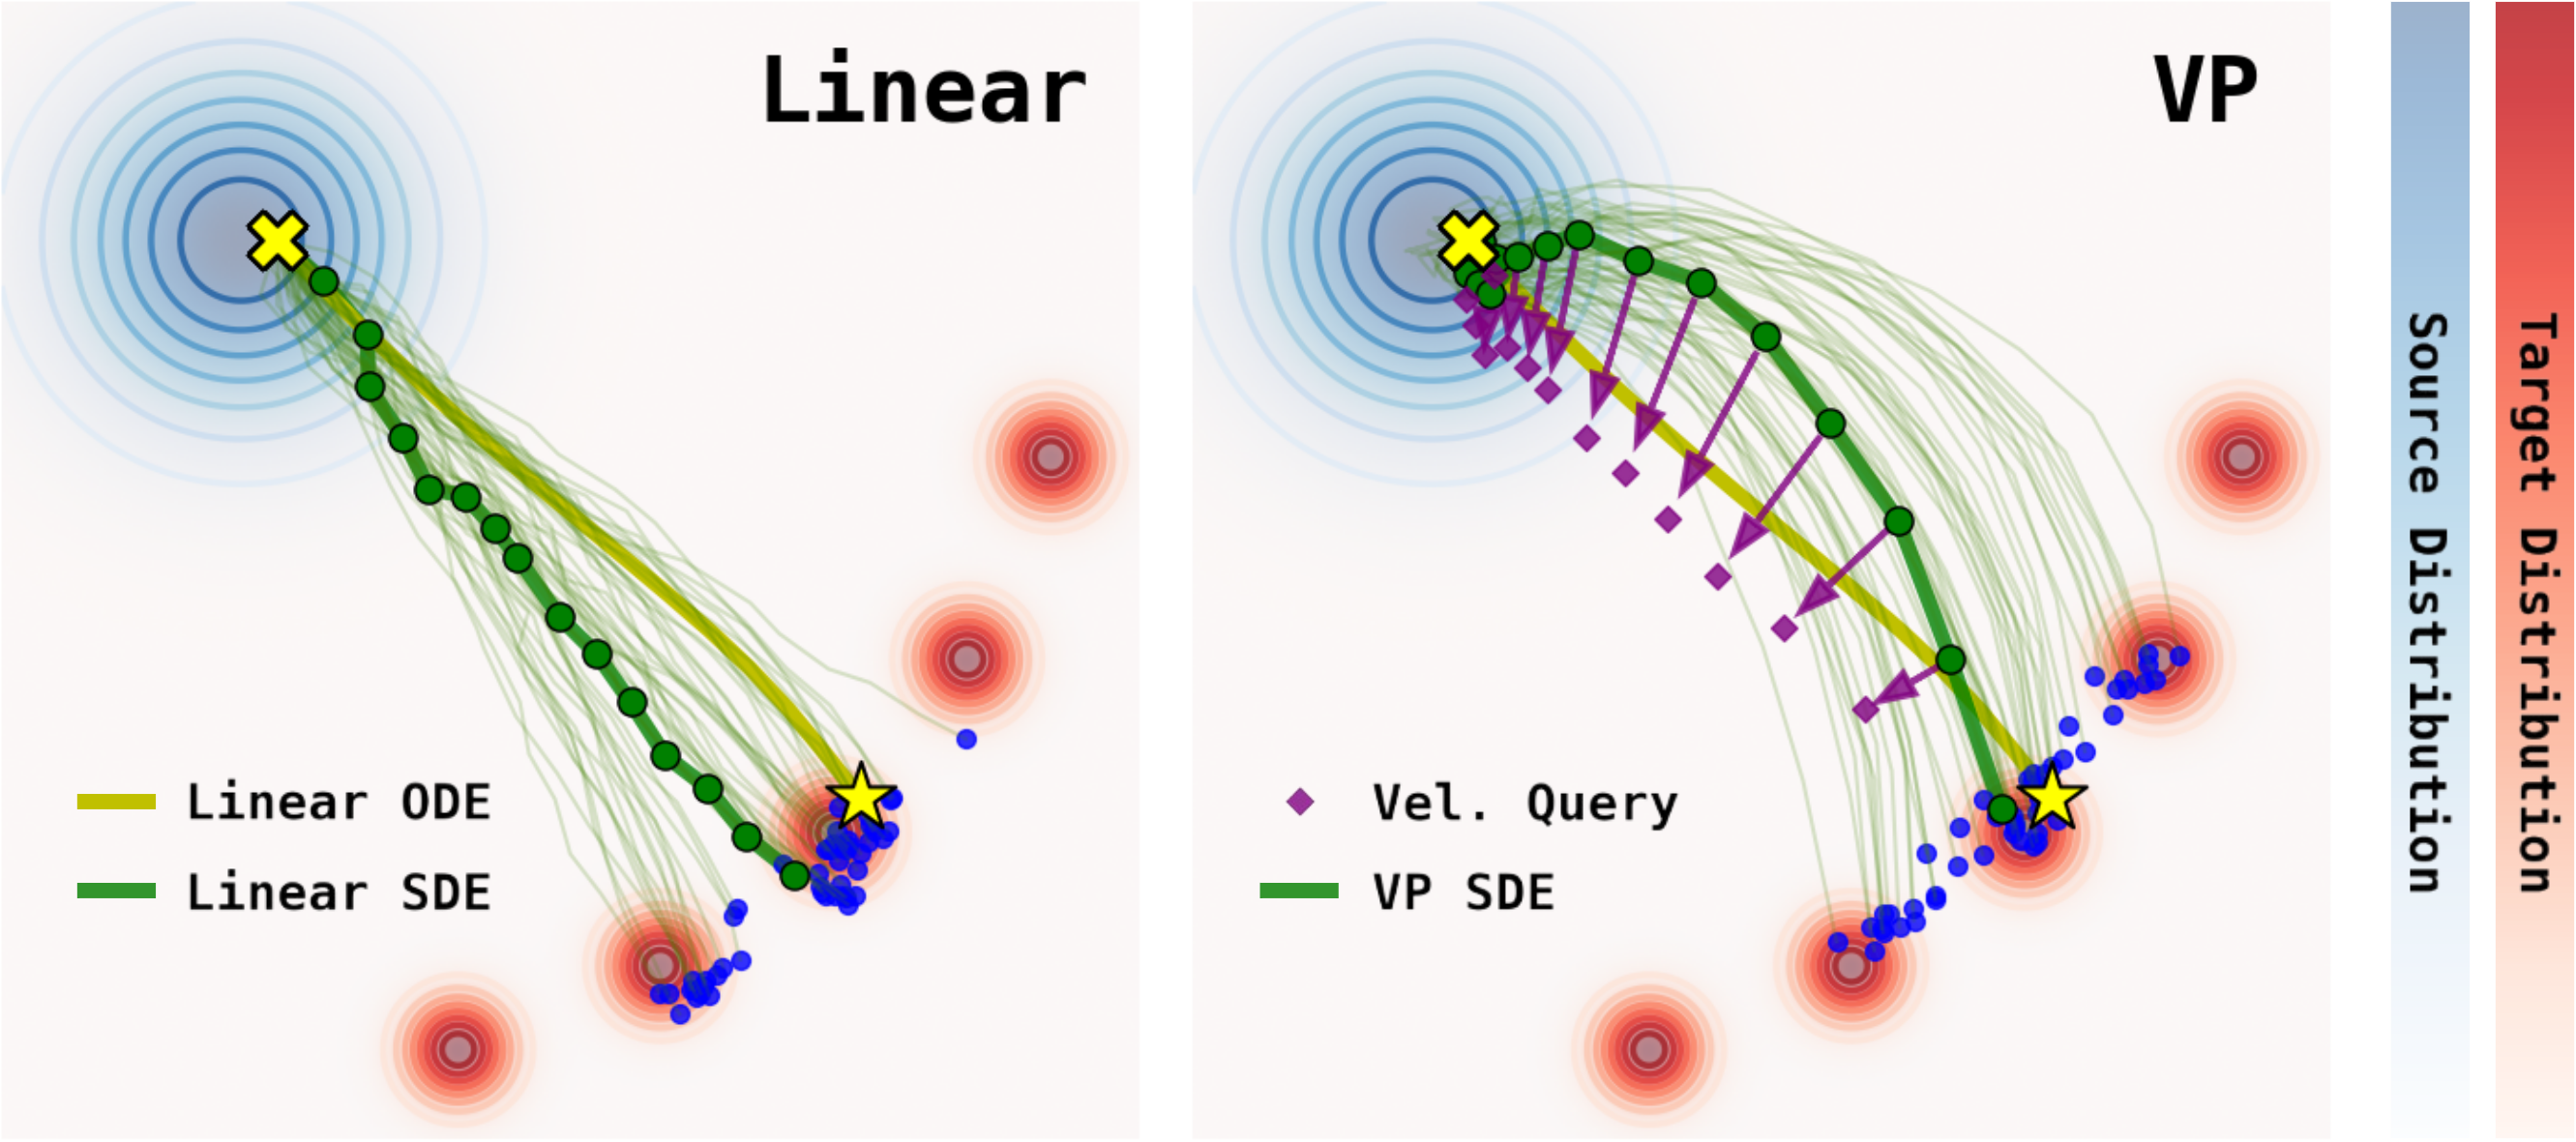
\includegraphics[width=\linewidth]{Figures/ode_sde_toy_visualization/Linear-VP.PNG}
%     \end{minipage}
%     \hfill
%     \begin{minipage}[t]{0.38\linewidth}
%         \small
%         \caption{\textbf{Comparison of Linear-SDE and VP-SDE.} Starting from the same initial noise latent, we generate $50$ samples using Linear-ODE, Linear-SDE, and VP-SDE. The visualization shows how trajectories evolve under different dynamics, highlighting differences in final sample distributions.}
%         \label{fig:ode_sde_viz}
%     \end{minipage}
% \end{figure}


\noindent 
\begin{figure}[t]
    \small
    \centering
    \begin{minipage}[t!]{0.48\linewidth}
        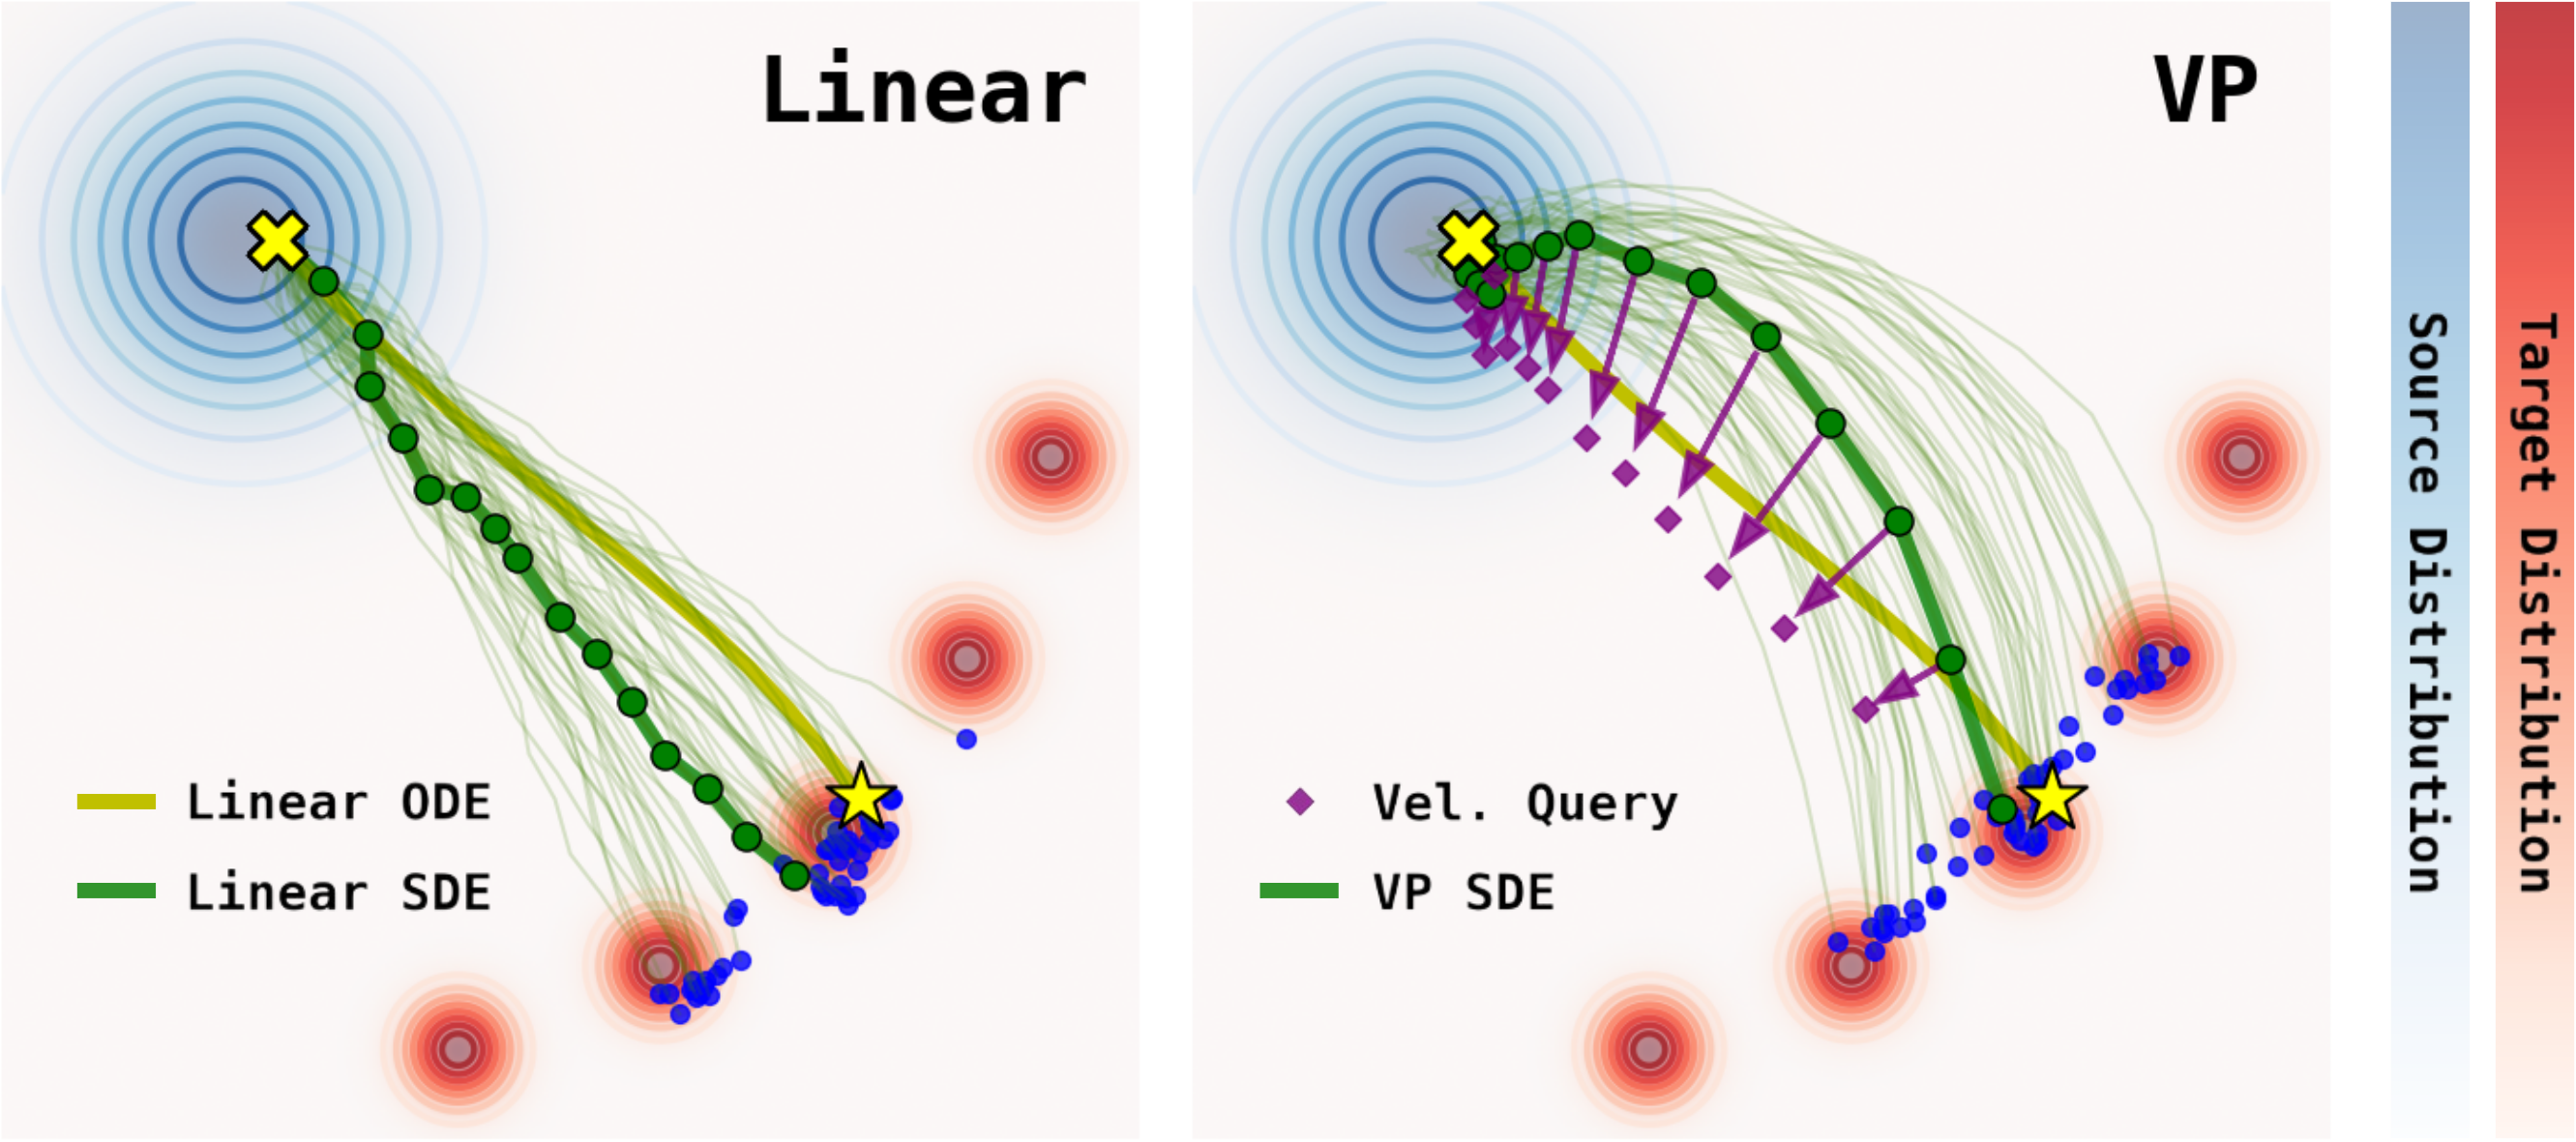
\includegraphics[width=\linewidth]{Figures/ode_sde_toy_visualization/Linear-VP.PNG}
        \caption{
            \textbf{Comparison of Linear-ODE, Linear-SDE, and VP-SDE.}
            The visualization shows how trajectories evolve under different dynamics starting from the same noise latent.
        }
        \label{fig:ode_sde_viz}
    \end{minipage}
    \hfill
    \begin{minipage}[t!]{0.48\linewidth}\vspace{-\topsep}
        {\scriptsize
        \setlength{\tabcolsep}{0.2em}
        \def\arraystretch{0.0}
        \newcolumntype{Z}{>{\centering\arraybackslash}m{0.32\linewidth}}
            \begin{tabularx}{\textwidth}{Z Z Z}
              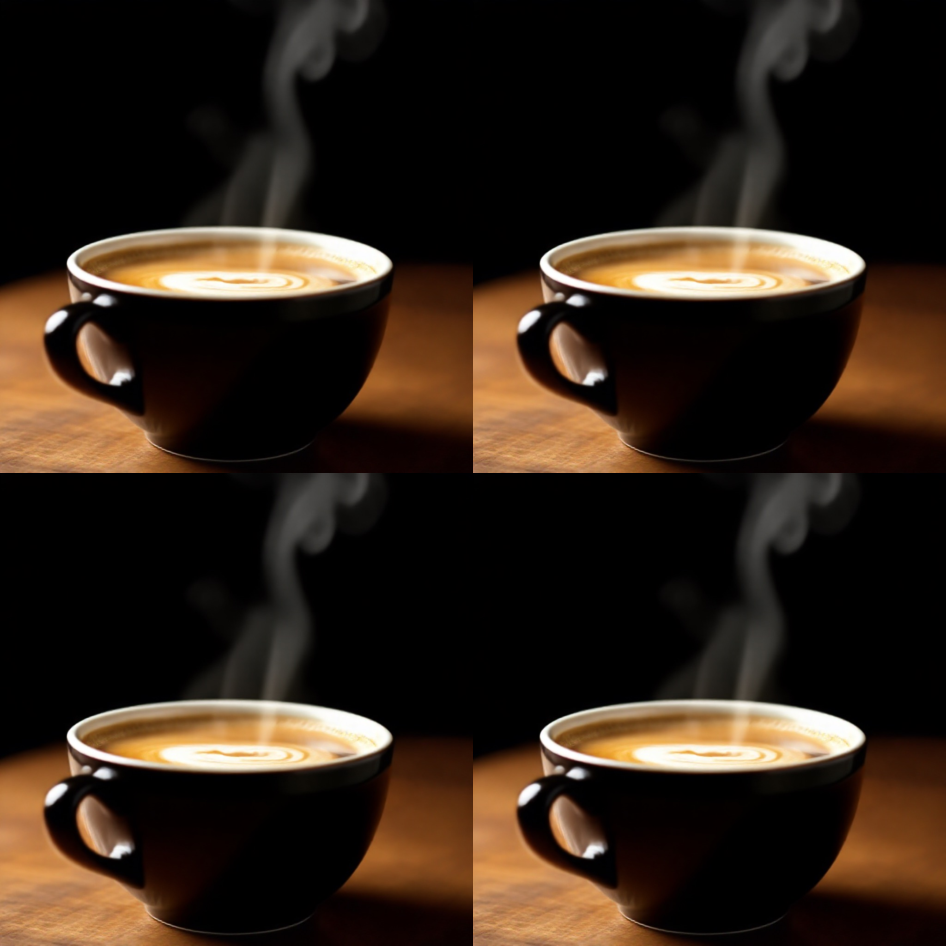
\includegraphics[width=\linewidth]{Figures/variance_test/linear_ode.pdf}
              &  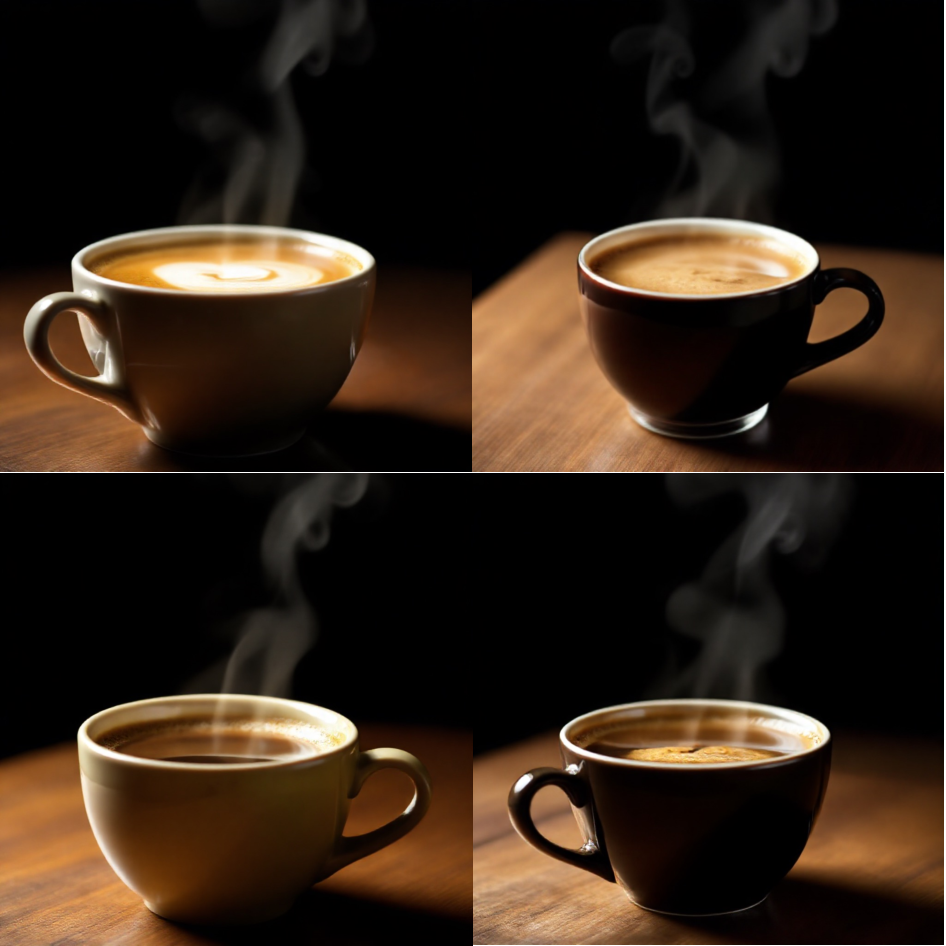
\includegraphics[width=\linewidth]{Figures/variance_test/linear_sde.pdf}
              &  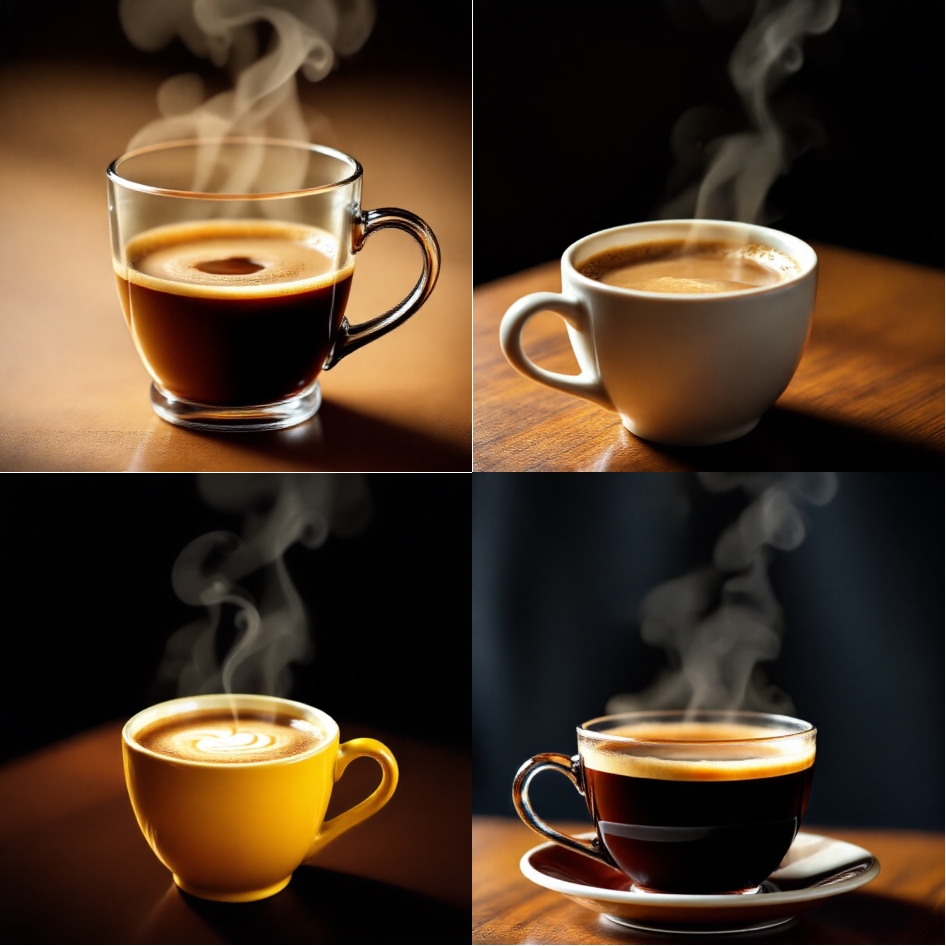
\includegraphics[width=\linewidth]{Figures/variance_test/vp_sde.pdf} \\
              \rule{0pt}{3ex} (a) Linear-ODE
              &
              \rule{0pt}{3ex} (b) Linear-SDE
              &
              \rule{0pt}{3ex} (c) VP-SDE \\
            \end{tabularx}
        }
        \captionof{figure}{
            \textbf{Sample diversity test using FLUX~\cite{BlackForestLabs:2024Flux} under linear and VP interpolant.} All samples share the same initial latent. Prompt: \textit{``A steaming cup of coffee''}.
        }
    \label{fig:variance_test}
    \end{minipage}
    \vspace{-1.1\baselineskip}
\end{figure}




% \begin{figure}
%     \centering
%     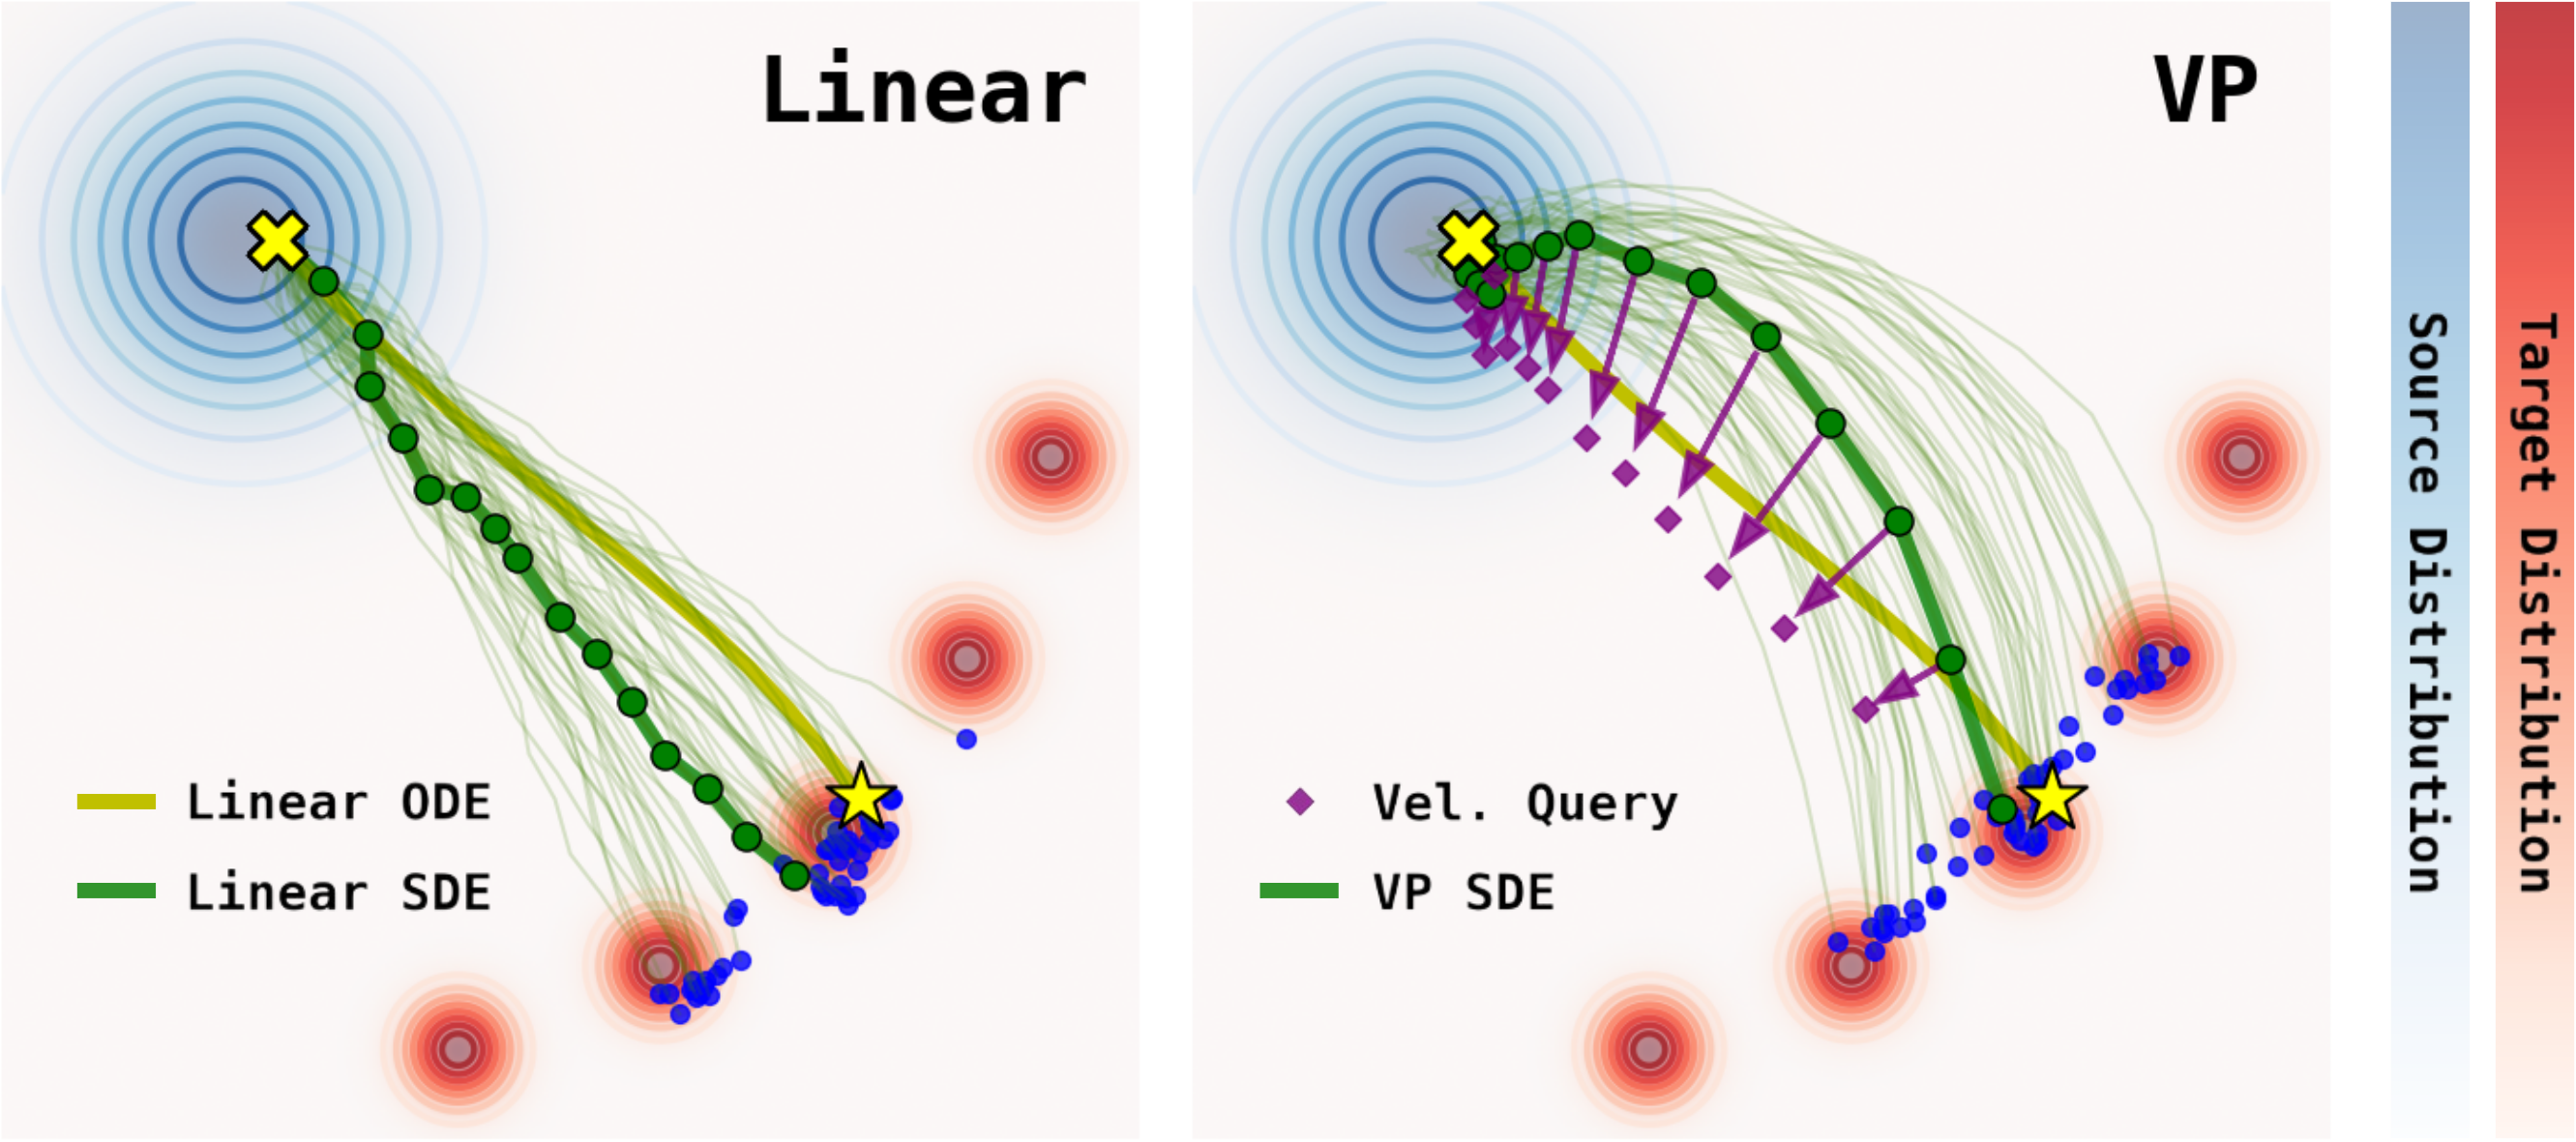
\includegraphics[width=\linewidth]{Figures/ode_sde_toy_visualization/Linear-VP.PNG}
%     \caption{\textbf{Comparison of Linear-SDE and VP-SDE}. Starting from the same initial noise latent, we generate $50$ samples using Linear-ODE, Linear-SDE, and VP-SDE.}
%     \label{fig:ode_sde_viz}
%     \vspace{-1.0\baselineskip}
% \end{figure}



% \begin{table}[!t]
%     \setlength{\tabcolsep}{2.9pt}
%     \centering
%     \small
%     \caption{\textbf{Stochastic interpolant scheduler}. $\beta_t$ is a predefined variance schedule~\cite{DDPM, Score based}.}
%     \label{tab:stochastic_interpolant}
%     % \vspace{-\baselineskip}
%     \newcolumntype{Z}{>{\centering\arraybackslash}m{0.3\linewidth}}
%     \newcolumntype{X}{>{\centering\arraybackslash}m{0.3\linewidth}}
%     \begin{tabular}{X | Z Z}
%         \multicolumn{3}{c}{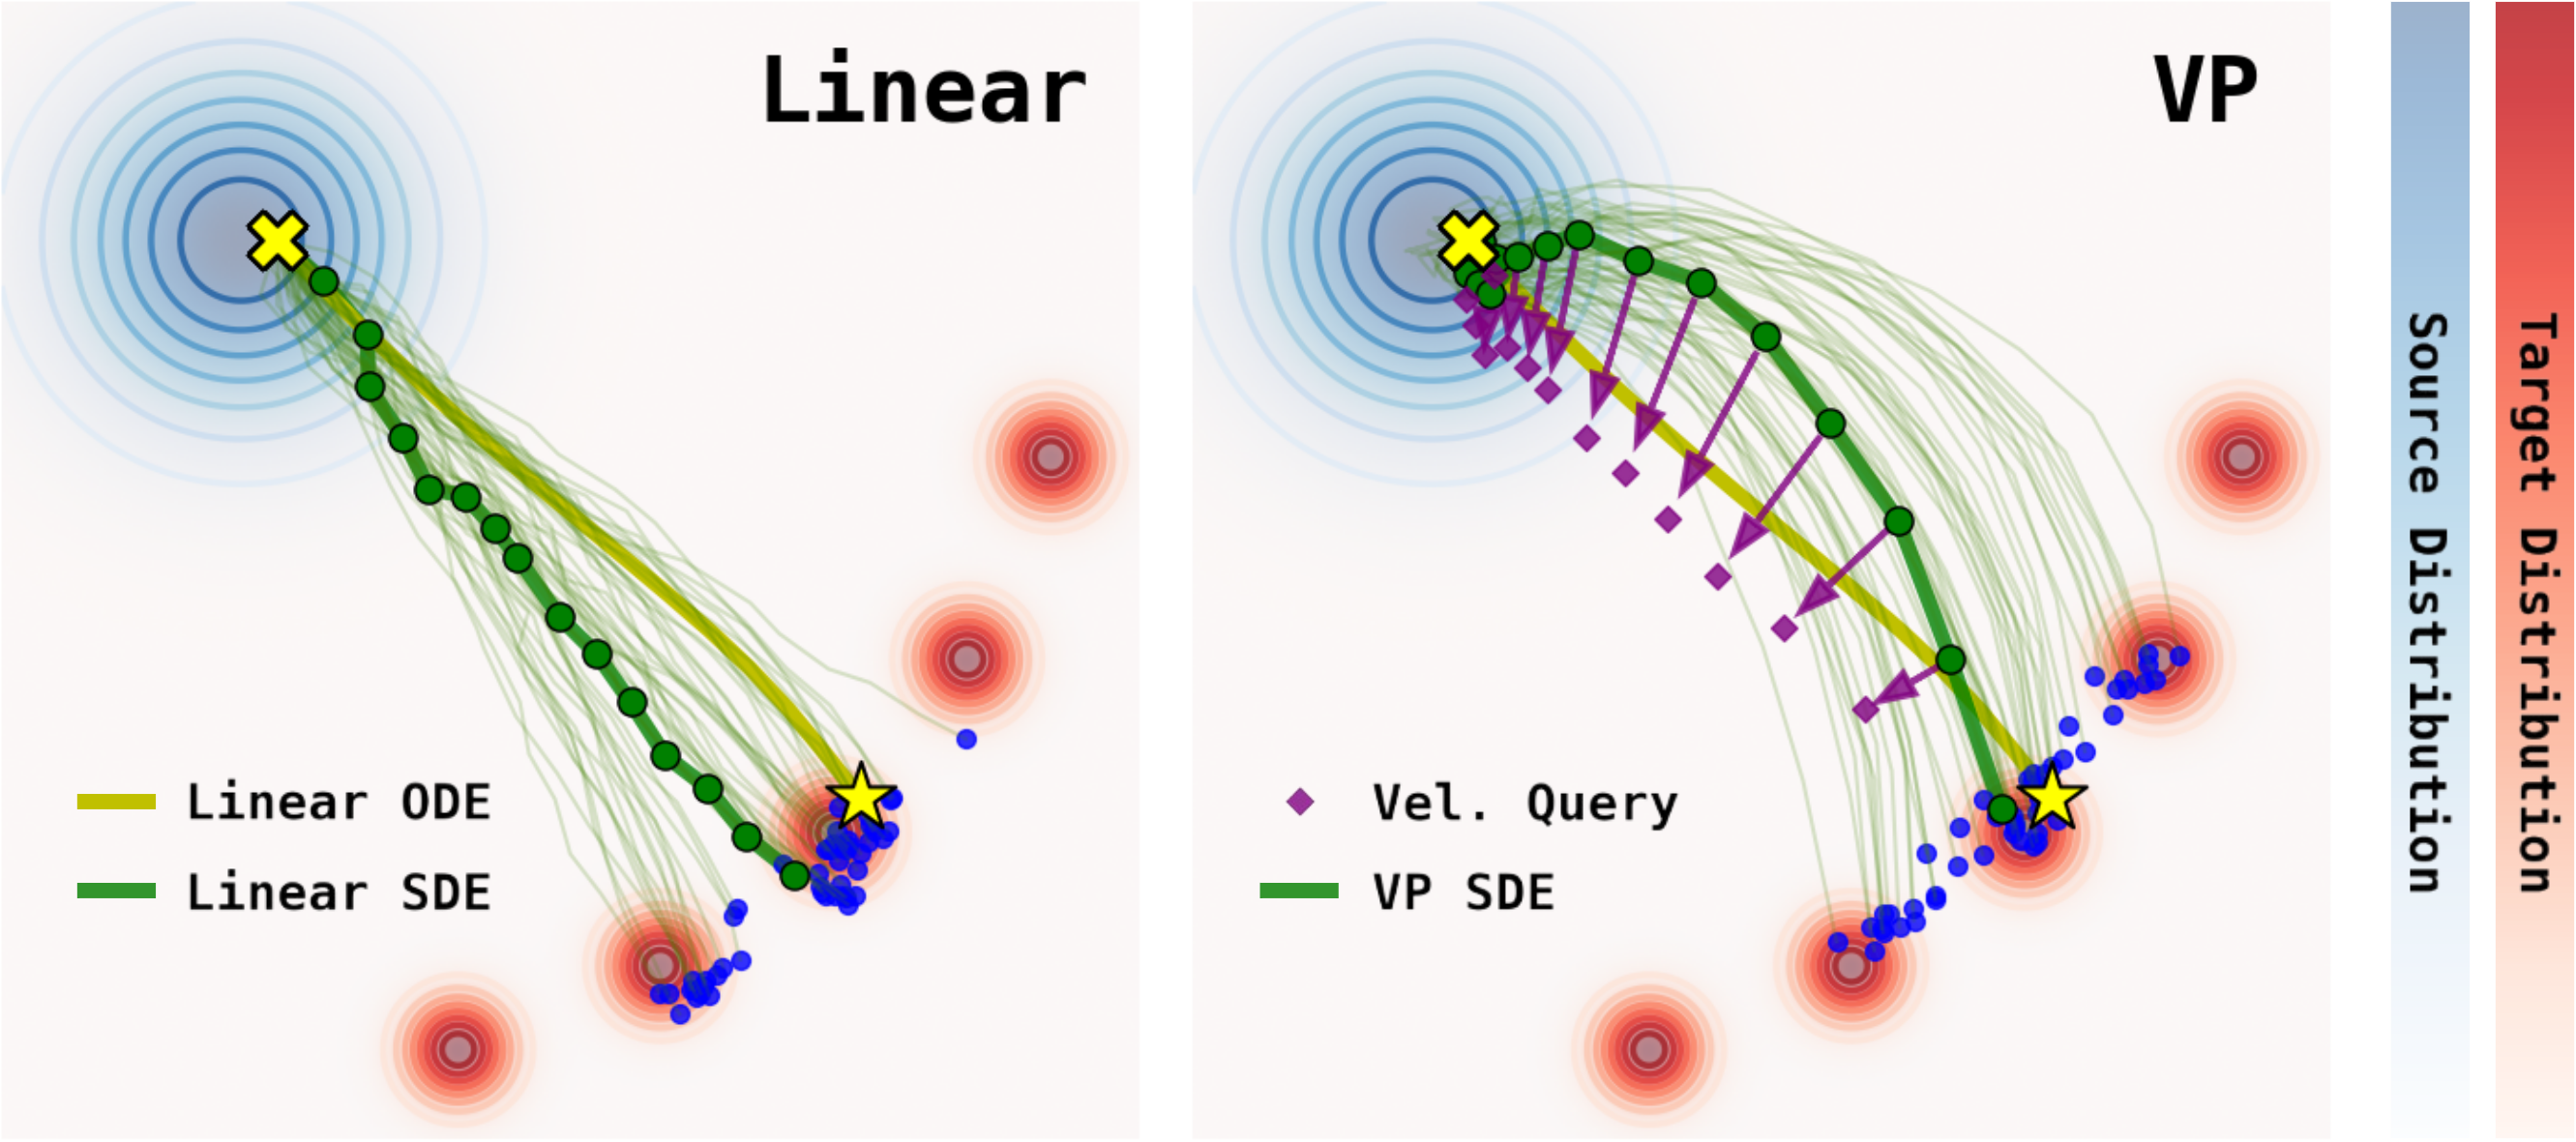
\includegraphics[width=\linewidth]{Figures/ode_sde_toy_visualization/Linear-VP.PNG}} \\
%         \toprule
%         Scheduler & $\alpha_t$ & $\sigma_t$ \\ 
%         \midrule
%         Linear & $1-t$ & $t$ \\
%         \midrule 
%         Variance Preserving & $\exp^{-\frac{1}{2} \int_0^t \beta_s ds}$ & $\sqrt{1 - \exp^{-\int_0^t \beta_s ds}}$ \\
%         \bottomrule
%     \end{tabular}
% \end{table}
